\documentclass[11pt]{article}
\usepackage[dvipsnames]{xcolor}
\usepackage{xcolor}
\usepackage{amsmath}
\usepackage{amssymb}
\usepackage{tikz}

\begin{document}

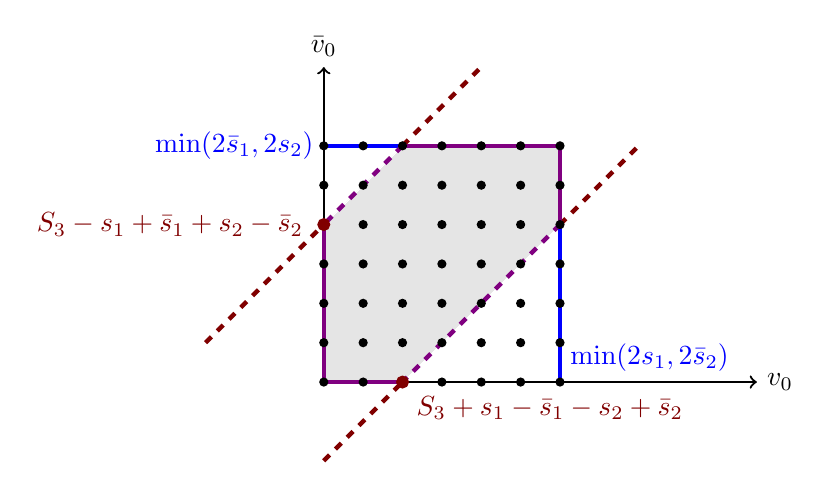
\begin{tikzpicture}[baseline={([yshift=-2ex]current bounding box.center)}]
    \draw[thick,->] (0,0) -- (0,3) node[left,Blue]{$\min(2\bar{s}_1,2s_2)$} -- (0,4) node[above]{$\bar{v}_0$};
    \draw[thick,->] (0,0) -- (3,0) node[above right,Blue]{$\min(2s_1,2\bar{s}_2)$} -- (5.5,0) node[right]{$v_0$};
    \draw[ultra thick,Blue] (3,0) -- (3,3) -- (0,3);
    \draw[ultra thick,dashed,Maroon] (-1.5,0.5) -- (0,2) (1,3) -- (2,4);
    \draw[ultra thick,dashed,Maroon] (0,-1) -- (1,0) (3,2) -- (4,3);

    \draw[line width=0,white,fill=gray!20] (1,3) -- (3,3) -- (3,2) -- (1,0) -- (0,0) -- (0,2) -- cycle;
    \draw[ultra thick,violet] (1,3) -- (3,3) -- (3,2) (0,2) -- (0,0) -- (1,0);
    \draw[ultra thick,violet,dashed] (1,3) -- (0,2) (3,2) -- (1,0);

    \foreach \x in {0,0.5,1,1.5,2,2.5,3}
    {
        \foreach \y in {0,0.5,1,1.5,2,2.5,3}
            \draw[ultra thick, fill=black!60] (\x,\y) circle (.8pt);
    };

    \draw[ultra thick,fill=Maroon,Maroon] (0,2) node[left]{$S_3-s_1+\bar{s}_1+s_2-\bar{s}_2 \ $} circle (1.5pt);
    \draw[ultra thick,fill=Maroon,Maroon] (1,0) node[below right=1pt]{$S_3+s_1-\bar{s}_1-s_2+\bar{s}_2$} circle (1.5pt);
\end{tikzpicture}

\end{document}